\chapter{Konzept}
\label{chap:konzept}


\section{Allgemein}

In diesem Abschnitt werden die grundlegenden Begriffe und der grobe Aufbau des Systems erläutert.

\textbf{Device} \\
Sensoren und Aktoren werden unter dem Begriff Device zusammengefasst.

\begin{figure}[H]
	\centering
		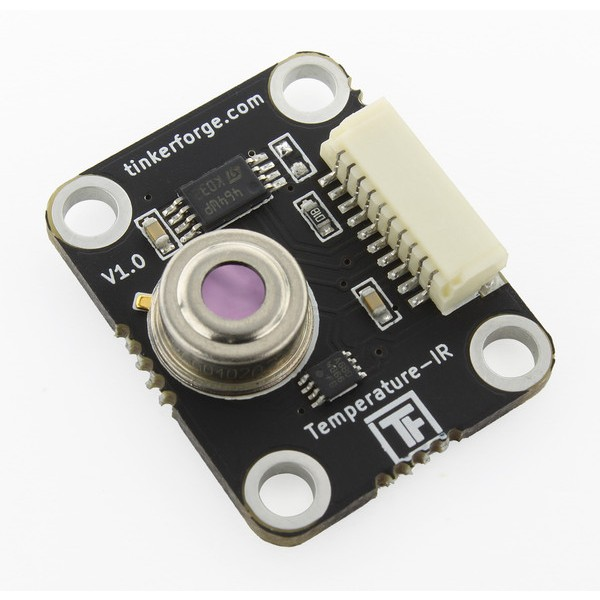
\includegraphics[width=0.3\textwidth]{bilder/bricklet_temperature_ir.jpg}
	\caption{Beispiel eines Devices: Tinkerforge Infrarot Temperatur Sensor}
\end{figure}


\textbf{Gateway} \\
Die einzelnen Devices eines \gls{iot} Systems sind an einen Gateway angeschlossen. Dies kann fix per Kabel oder über eine Drahtlosschnittstelle wie z. Bsp. Bluetooh umgesetzt sein. Typsicherweise werden Kleincomputer (Single Board Computer) wie ein Raspberry Pi oder Intel Galileo eingesetzt. Diese Geräte zeichen sich aus durch sehr kompakte Bauform (Kreditkatenformat) und bieten trotzdem genügend Ressourcen um darauf hardwareunahängige Anwendungen (z. Bsp. Java, Python, Javascript) laufen zu lassen. 
Ein Gateway führt die Daten der einzlenen Sensoren zusammen und vereinheiltliche die Formate der Daten. Ausserdem übernimmt er die Kommunikation mit der Aussenwelt, indem er eine Verbindung zum zentralen Broker herstellt.

\begin{figure}[H]
	\centering
		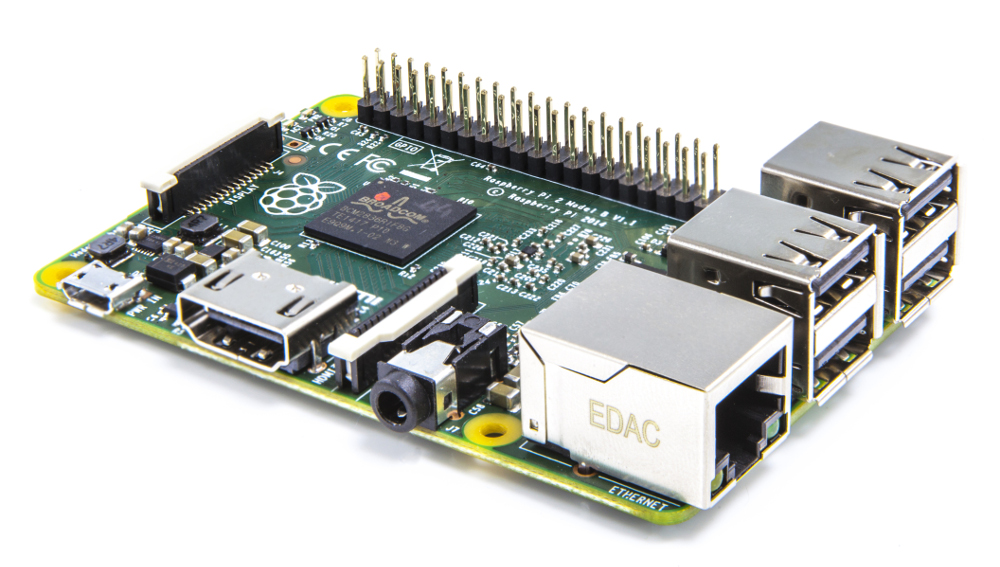
\includegraphics[width=0.6\textwidth]{bilder/raspi_2.jpg}
	\caption{Beispiel eines Gateways: Raspberry Pi 2}
\end{figure}

\textbf{MQTT-Broker} \\
Der Broker ist bei \acrshort{a_mqtt} Anwendungen von zentraler Bedeutung, da alle Daten via Broker zwischen den Teilnehmern ausgetauscht werden. Pro System gibt es typischeise einen Broker. Dieser muss für alle Teilnehmener (Gateways und Applikationen) einfach zu erreichen sein und muss eine hohe Verfügbarkeit aufweisen.

\textbf{Applikation} \\
Es können grundsätzlich beliebige Applikationen auf allen gängigen Plattformen und Technologien mit den System kommunizieren. Die einzige Grundbedingung ist, dass die Applikation \acrshort{a_mqtt} fähig ist, was sich durch das Einbinden der entsprechenden Libraries einfach realisieren lässt.
\\


Bei der Beschreibung eines einzelnen Devices werden folgende drei Bereiche unterschieden:

\textbf{State} \\
Die Menge aller Eigenschaften des Devices und deren Werte wird als State bezeichnet. Beispielsweise Name, Firmwareversion, etc. Der State eines Devices ist beständig, d.h. solange keine Interaktion geschieht, verändert sich der State nicht.


\textbf{Events} \\
Tritt auf dem Device ein Ereignis ein, wird dadurch ein Event erzeugt. Ein Event wird grundsätzlich vom Device selbst ausgelöst. Beispielsweise erzeugt ein Temperatursensor alle 5 Sekunden ein Event welches den Messwert enthält. Applikationen registrieren sich, um bestimmte Events von den Devices zu erhalten.


\textbf{Commands} \\
Eine Applikation interagiert mit einem Device, indem Commands an eines oder mehrere Devices gesendet werden. Die Devices empfangen die Commands und reagieren entsprechend. Ein Command ist bestimmt durch einen Namen und Parameter mit dazugehörigen Werten. 
Beispielsweise kann bei einem Temperatursensor über einen Command \code{SetInterval: 10s} der Abstand der Messungen eingestellt werden.
Ein Device muss bekanntgeben, auf welche Commands mit welchen Paramtern es reagiert.


\begin{figure}[H]
	\centering
		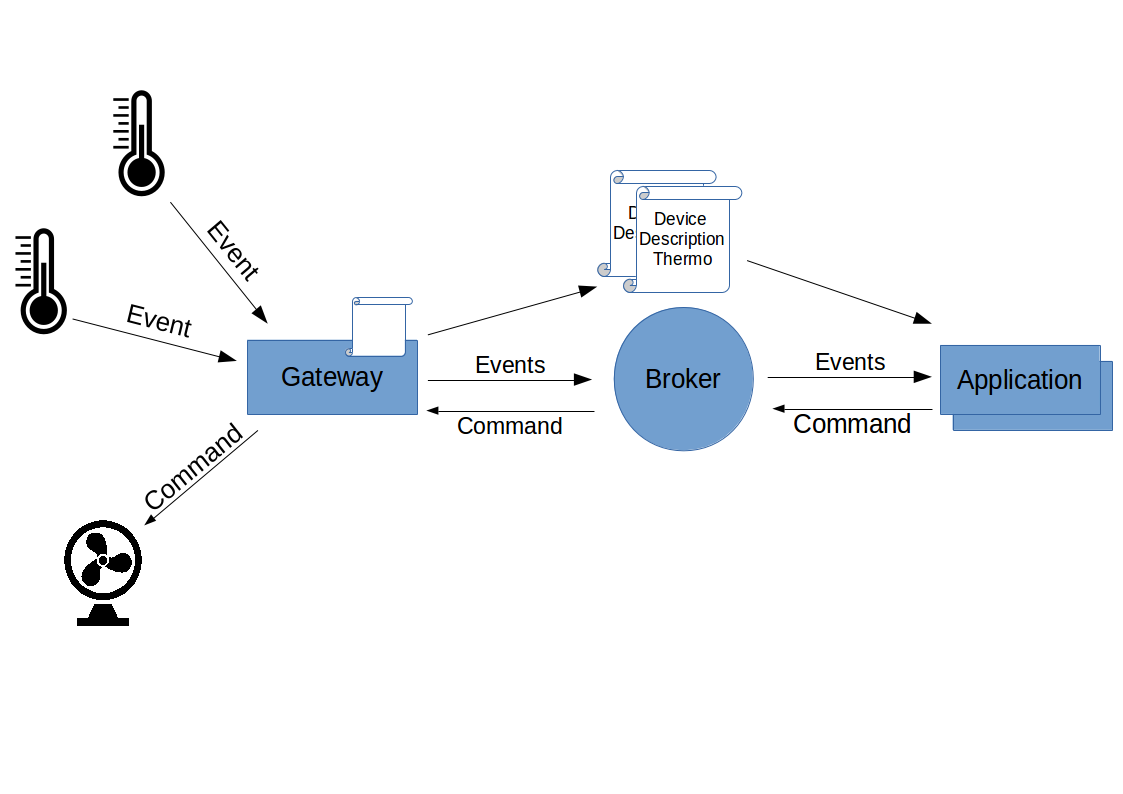
\includegraphics[width=0.8\textwidth]{diag/Overview.png}
	\caption{\label{fig:overview}Übersicht der}
\end{figure}


\section{Hierarchie Topics}


Die Topic Hiearachie wird nach folgenden Muster aufgebaut:

\begin{figure}[H]
	\centering
		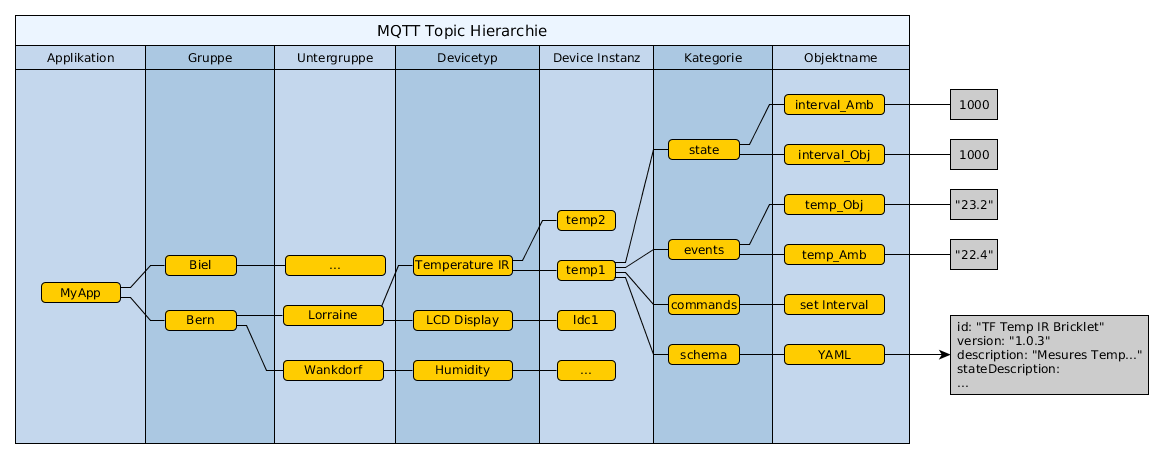
\includegraphics[width=1.0\textwidth]{diag/topic_hierarchy.png}
	\caption{\label{fig:tempitTopics}Aufbau MQTT Topics mit Beispieldaten}
\end{figure}
TODO: farben, was fix, was variabel

\begin{table}[H]
\begin{tabularx}{\textwidth}{|l|X|l|}

 \hline
 {\bf Level } & {\bf Beschreibung } & {\bf Beispiel } \\ 
 \hline
 0  &   \textbf{Applikation} \newline Identifikation der Anwendung.  &    
  thesisDemo   \\ \hline
 
 1  &   \textbf{Gruppe}  \newline Gruppierung der Devices auf Stufe 1, beispielsweise nach Standort  &     - Bern  \\ \hline

 2  &   \textbf{Untergruppe} \newline Gruppierung der Devices auf Stufe 2, beispielsweise nach Quartier   &   - Lorraine  \\ \hline

 3  &   \textbf{Devicetyp} \newline Bezeichnung, um was für einen Typ von Sensor oder Aktor es sich handelt.  &   Temperatursensor   \\ \hline

 4  &   \textbf{Device Instanz} \newline Da mehrere Devices vom selben Typ im Einsatz sein können, wird auf dieser Stufe mit einer eindeutigen ID der konkrete Sensor resp. Aktor angegeben.   &    temp001   \\ \hline
 
 5  &   \textbf{Kategorisierung Devicedaten} \newline  Die Eigenschaften und Daten werden in die nachfolgenden Teile aufgegliedert.  &     events, state, commands, schema   \\ \hline
 
 6  &   \textbf{Objektname} \newline Name es State, Events oder Commands \newline     &     Temperatur   \\ \hline

 6  &   \textbf{Schema Format} \newline Falls es sich um ein Unterobjekt von 'schema' handelt, wird hier das Format des Schemas angegeben   &     YAML, JSON   \\ \hline
 

\end{tabularx}
\caption{Topic Hierarchie}
\end{table}


